Via de simples calculs d'aires, il est très facile de découvrir les classiques identités remarquables
$(a + b)^2 = a^2 + b^2 + 2ab$,
$(a - b)^2 = a^2 + b^2 - 2ab$
et
$(a + b)(a - b) = a^2 - b^2$.
%
Par exemple, en considérant le dessin ci-dessous où $ABCD$, $AEGF$ et $GHCK$ sont des carrés,
il est évident que $(a + b)^2 = a^2 + b^2 + 2 ab$.
Malheureusement, cette démonstration n'est valable que pour $a > 0$ et $b > 0$ \emph{(ce sont des contraintes géométriques concrètes)}.

\begin{center}
	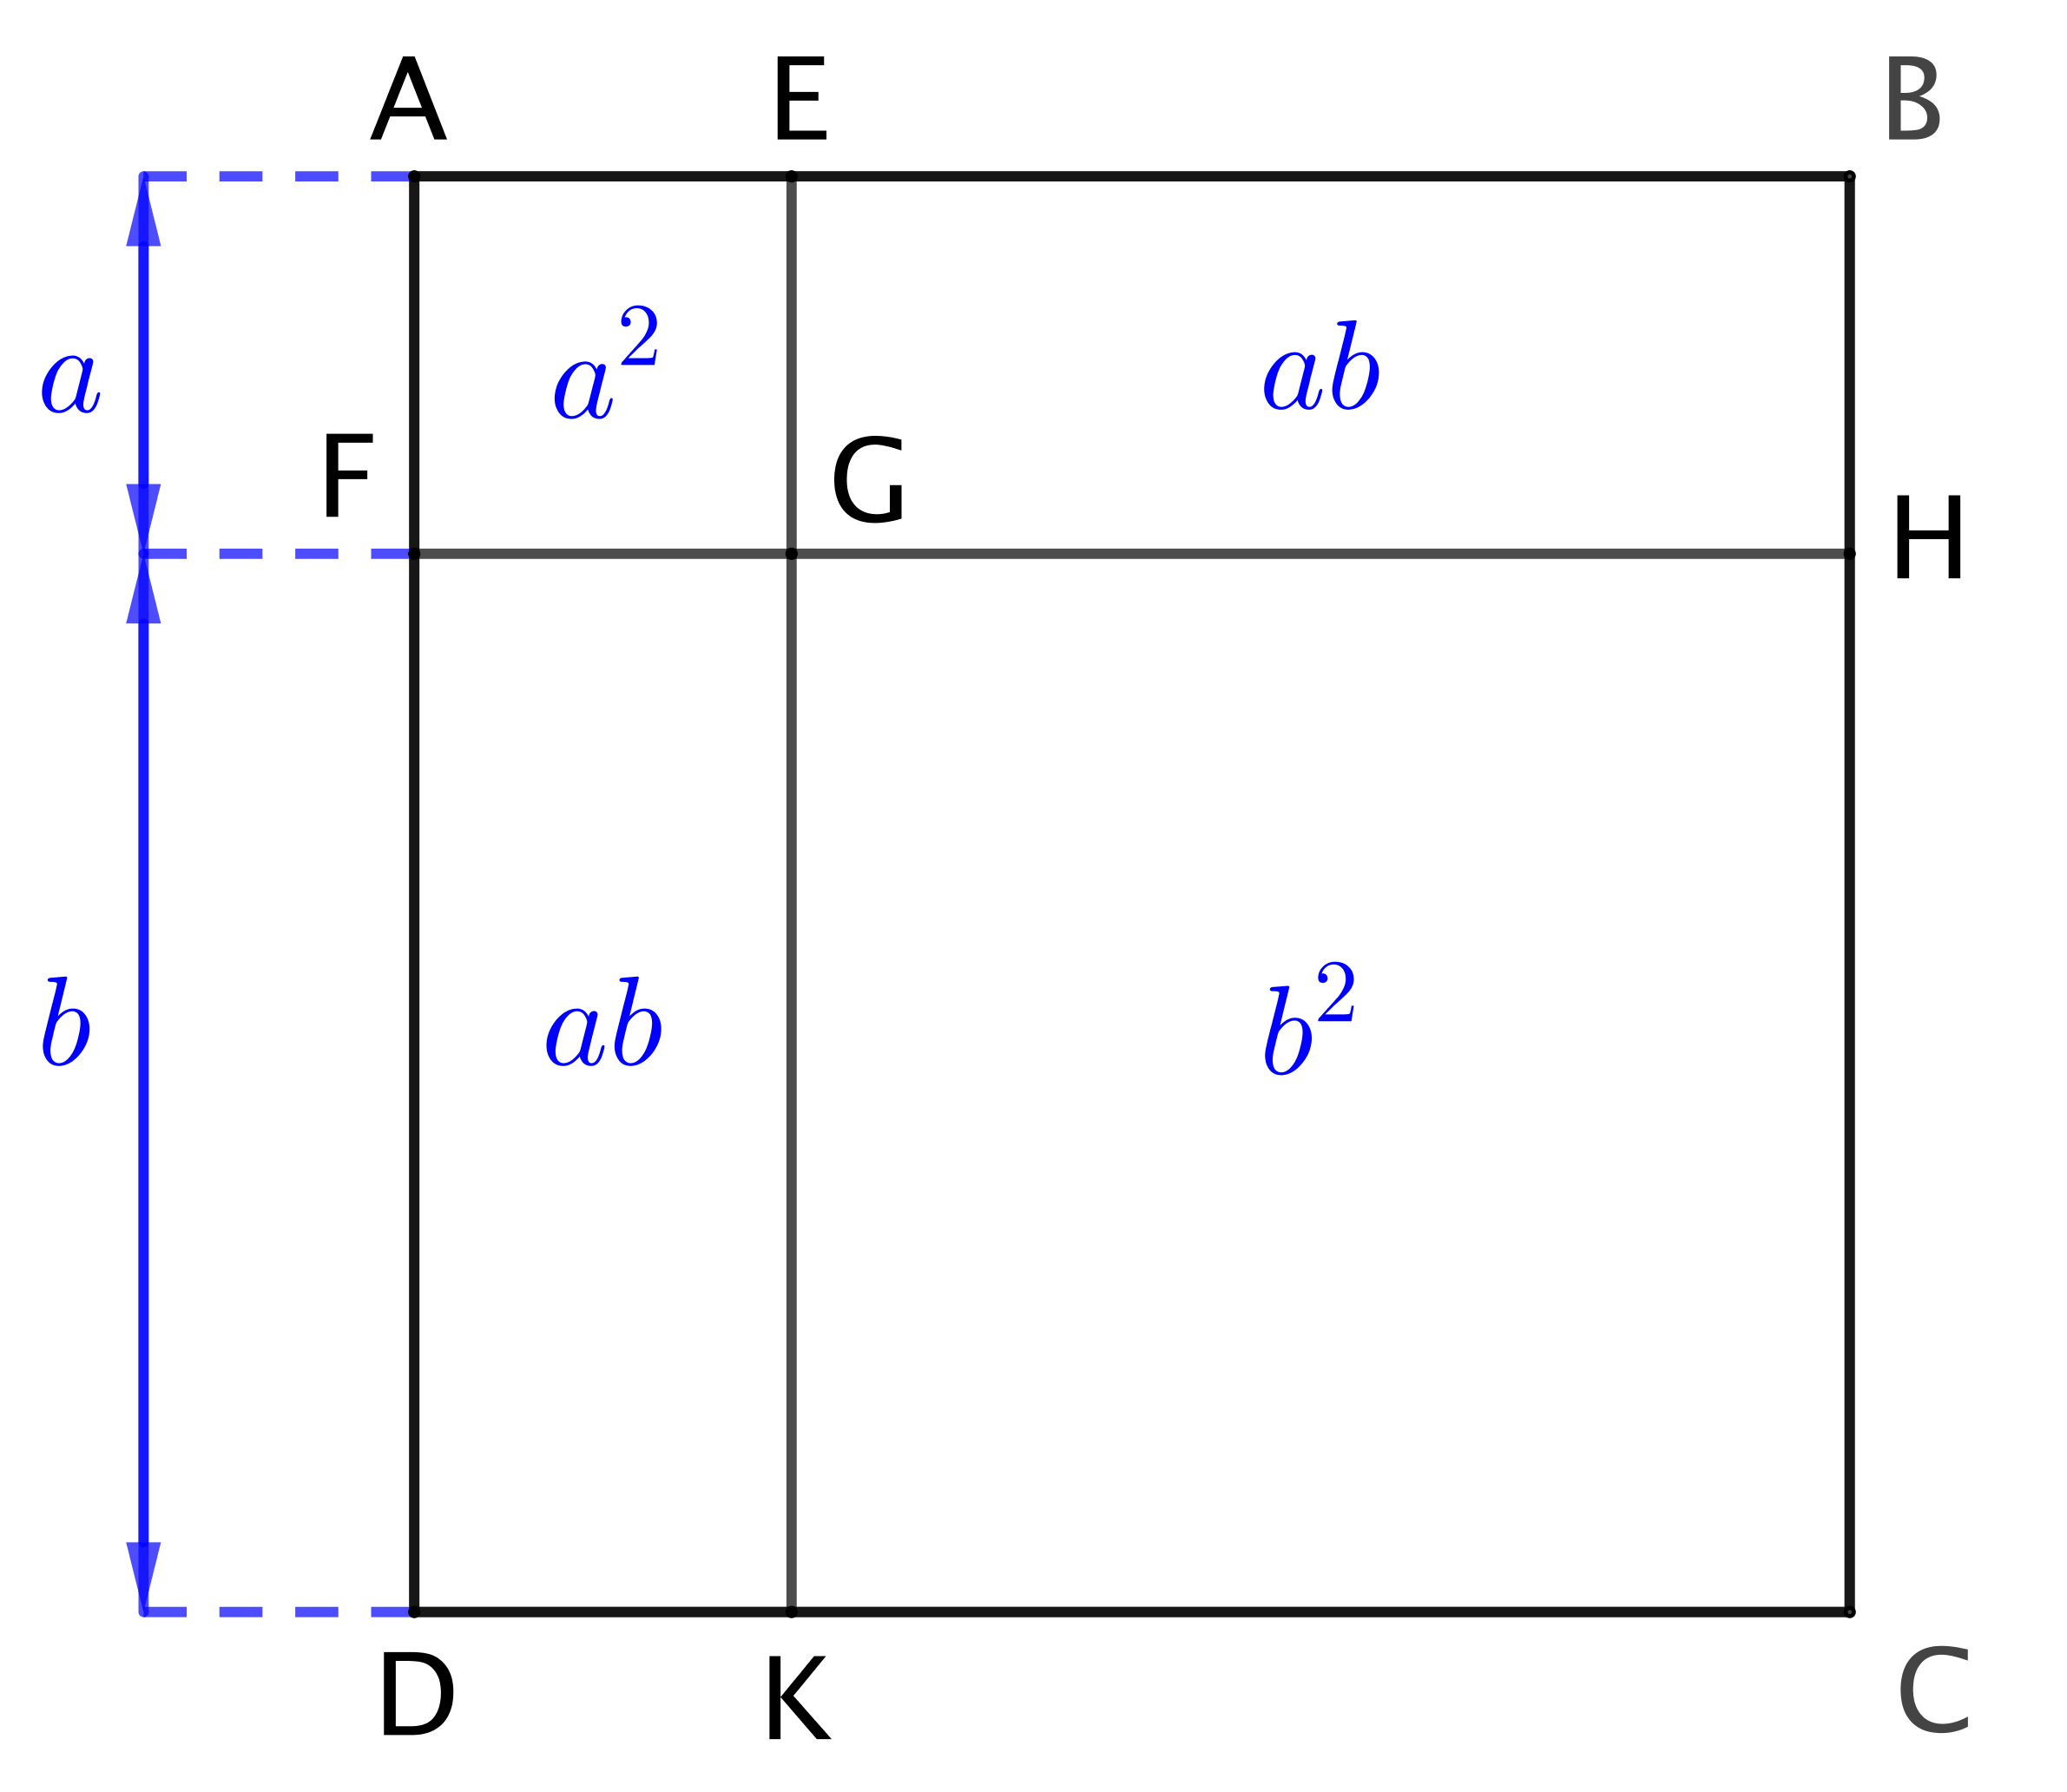
\includegraphics[scale = .7]{(a+b)^2.png}
\end{center}


Comment passer à $(a + b)^2 = a^2 + b^2 + 2 ab$ pour $a$ et $b$ deux réels de signes quelconques ?
Classiquement, on fait une vérification via un calcul algébrique: en résumé, on conjecture géométriquement, puis on valide algébriquement.
%
Bien que rigoureuse, la démarche précédente est peu satisfaisante, car elle balaye d'un revers de main l'approche géométrique, dont le rôle est réduit à la découverte d'une formule.
Si l'on considère le dessin ci-après, il est dommage de devoir faire du calcul algébrique pour valider $(a + b + c)^2 = a^2 + b^2 + c^2 + 2 ab + 2 ac + 2 bc$ pour $a$, $b$ et $c$ des réels de signes quelconques.
Ce serait bien de pouvoir passer directement de $(a + b + c)^2 = a^2 + b^2 + c^2 + 2 ab + 2 ac + 2 bc$ vraie pour $a > 0$, $b > 0$ et $c > 0$, à la validation de l'identité pour $a$, $b$ et $c$ de signes quelconques.

\begin{center}
	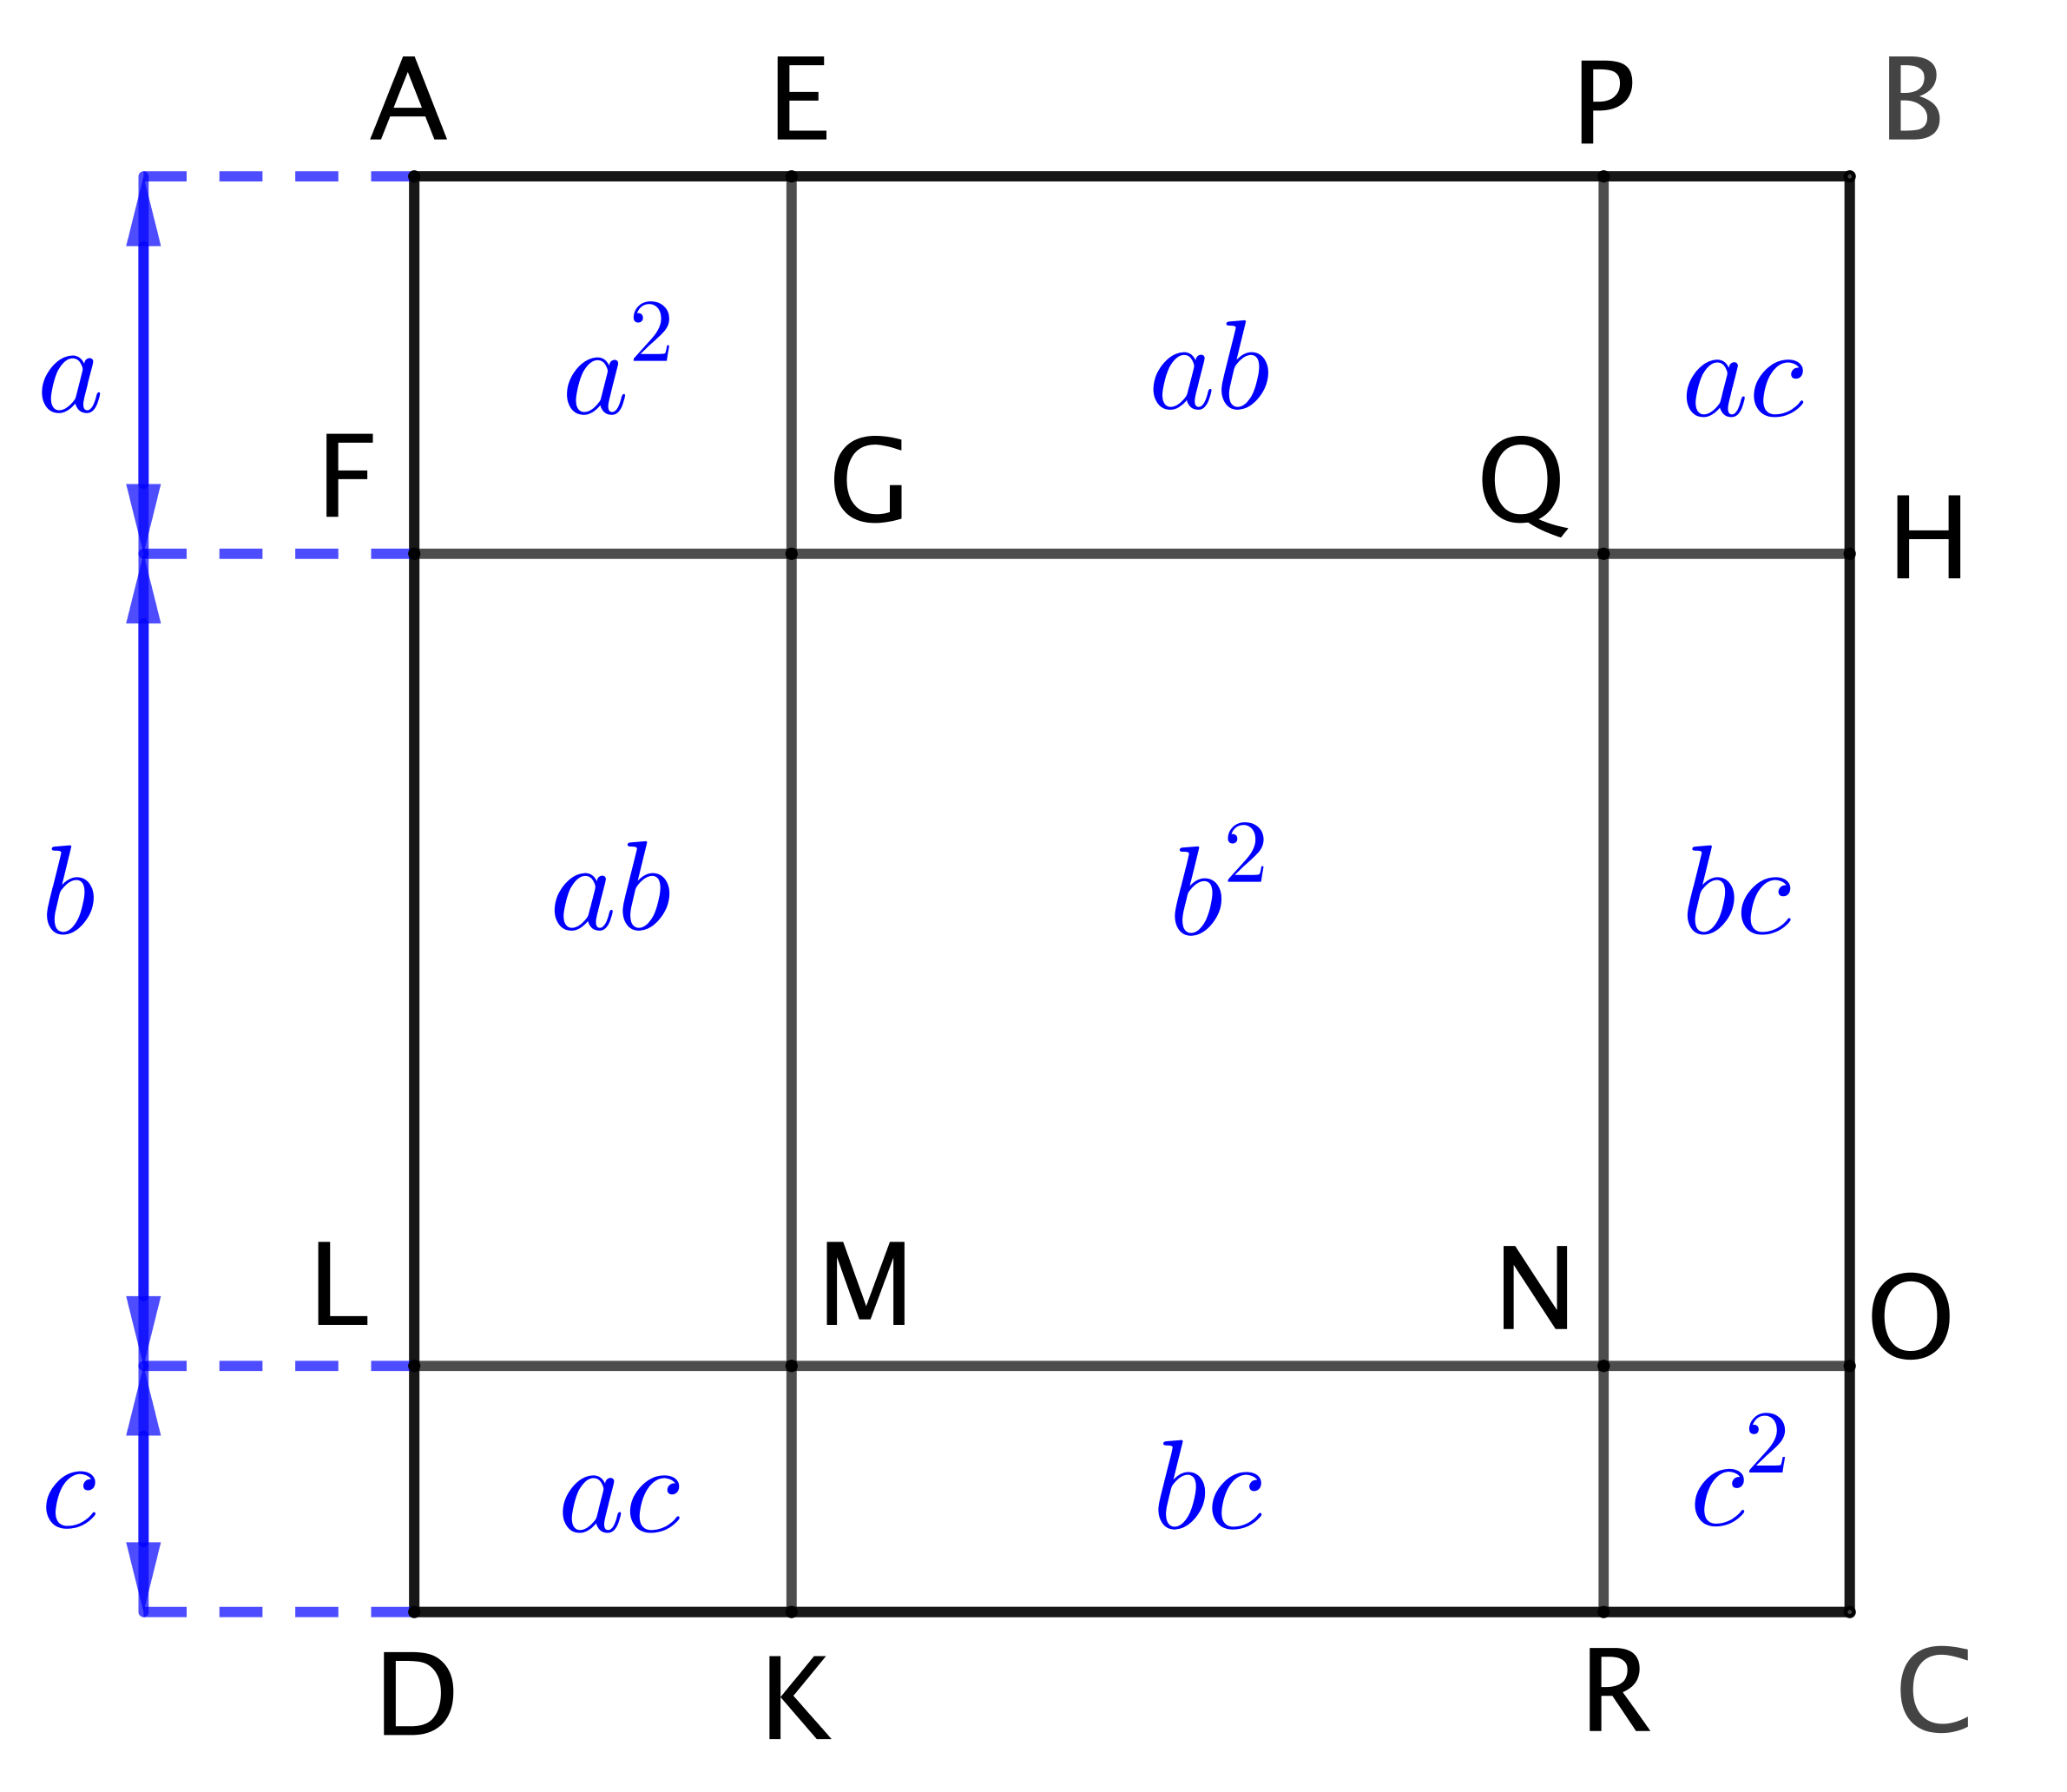
\includegraphics[scale = .7]{(a+b)^3.png}
\end{center}

Le fait \ref{poly-nullity-pos} ci-après va rendre licite le passage des formules géométriques contraintes précdentes au cas général en faisant les choix suivants.
%
\begin{itemize}[label=\small\textbullet]
	\item $p(a ; b) = (a + b)^2 - a^2 - b^2 - 2 ab$

	\item $p(a ; b ; c) = (a + b + c)^2 - a^2 - b^2 - c^2 - 2 ab - 2 ac - 2 bc$
\end{itemize}


% ----------- %


\begin{fact} \label{poly-nullity-pos}
	Soit $p: \RR^n \rightarrow \RR$ une fonction polynomiale à $n$ variables, où $n \in \NNs$.
	Si $p$ s'annule sur $\big( \RRsp \big)^n$, alors $p$ s'annule sur $\RR^n$ tout entier. 
\end{fact}


\begin{proof}
	Raisonnons par récurrence sur $n \in \NNs$ pour démontrer la validité de la propriété $\setproba{P}(n)$ définie par
	\emph{\og 
		Pour tout fonction polynomiale réelle $p: \RR^n \rightarrow \RR$,
		si $p$ s'annule sur $\big( \RRsp \big)^n$,
		alors $p$ s'annule sur $\RR^n$ tout entier. 
	\fg}\kern2pt.
	%
	\begin{itemize}[label=\small\textbullet]
		\item \textbf{Cas de base.}
		%
		$\setproba{P}(1)$ signifie qu'une fonction polynomiale réelle à une variable s'annulant sur $\RRsp$ est identiquement nulle sur $\RR$ tout entier.
		%
		Comme un polynôme réel non nul n'a qu'un nombre fini de racines, nous avons la validité de $\setproba{P}(1)$.


		\item \textbf{Hérédité.}
		%
		Supposons $\setproba{P}(n)$ valide pour un naturel $n$ quelconque.
		Soit une fonction polynomiale $p$ à $(n + 1)$ variables vérifiant les conditions de la propriété $\setproba{P}(n + 1)$.
		%
		\begin{enumerate}
		    \item Soient $x \in \RRsp$ fixé, puis la fonction polynomiale $p_x(x_1 ; ... ; x_n) = p(x_1 ; ... ; x_n ; x)$.
		    Comme $p_x$ vérifie les conditions de la propriété $\setproba{P}(n)$, par hypothèse de récurrence, on a
		    $p_x(x_1 ; ... ; x_n) = 0$, soit $p(x_1 ; ... ; x_n ; x) = 0$, pour tous réels $x_1$ , ... , $x_n$.


		    \item Fixons maintenant des réels $x_1$ , ... , $x_n$ de signes quelconques, et considérons la fonction polynomiale $\ell(x) = p(x_1 ; ... ; x_n ; x)$.
		    Le point précédent montre que $\ell$ vérifie $\setproba{P}(1)$, donc $\ell(x) = 0$, soit $p(x_1 ; ... ; x_n ; x) = 0$, pour tout réel $x$, d'après le cas de base.


		    \item Finalement, $p(x_1 ; ... ; x_n ; x) = 0$ pour tous réels $x_1$ , ... , $x_n$ et $x$.
		    Autrement dit, nous avons déduit la validité de $\setproba{P}(n+1)$ à partir de celle de $\setproba{P}(n)$.
		\end{enumerate}
		
		
		\item \textbf{Conclusion.}
		%
		Par récurrence sur $n \in \NNs$, la propriété $\setproba{P}(n)$ est vraie pour tout naturel non nul $n$.
	\end{itemize}

	\null\vspace{-6ex}
\end{proof}


% ----------- %


\begin{example}
	En utilisant une approche géométrique semblable à celle présentée plus haut, il devient évident, et rigoureux maintenant, d'affirmer que $\forall n \in \NNs$, $\forall (a_1 ; ... ; a_n) \in \RR^n$, on a :
\[
	\big( \sum_{k=1}^{n}a_k \big)^2
	=
	\sum_{k=1}^{n} \left( a_k \right)^2
	+
	2 \sum_{1 \leq i < j \leq n} a_i a_j
\]
\end{example}


% ----------- %


\begin{example}
	Nous laissons le soin au lecteur de vérifier à l'aide d'un cube, le solide géométrique, la validité de l'identité $(a + b)^3 = a^3 + 3 a^2 b + 3 a b^2 + b^3$ pour tous réels $a$ et $b$.
\end{example}


% ----------- %


Considérons maintenant le dessin ci-dessous avec $d = a - b$, et la contrainte $a > b$.
%
\begin{center}
	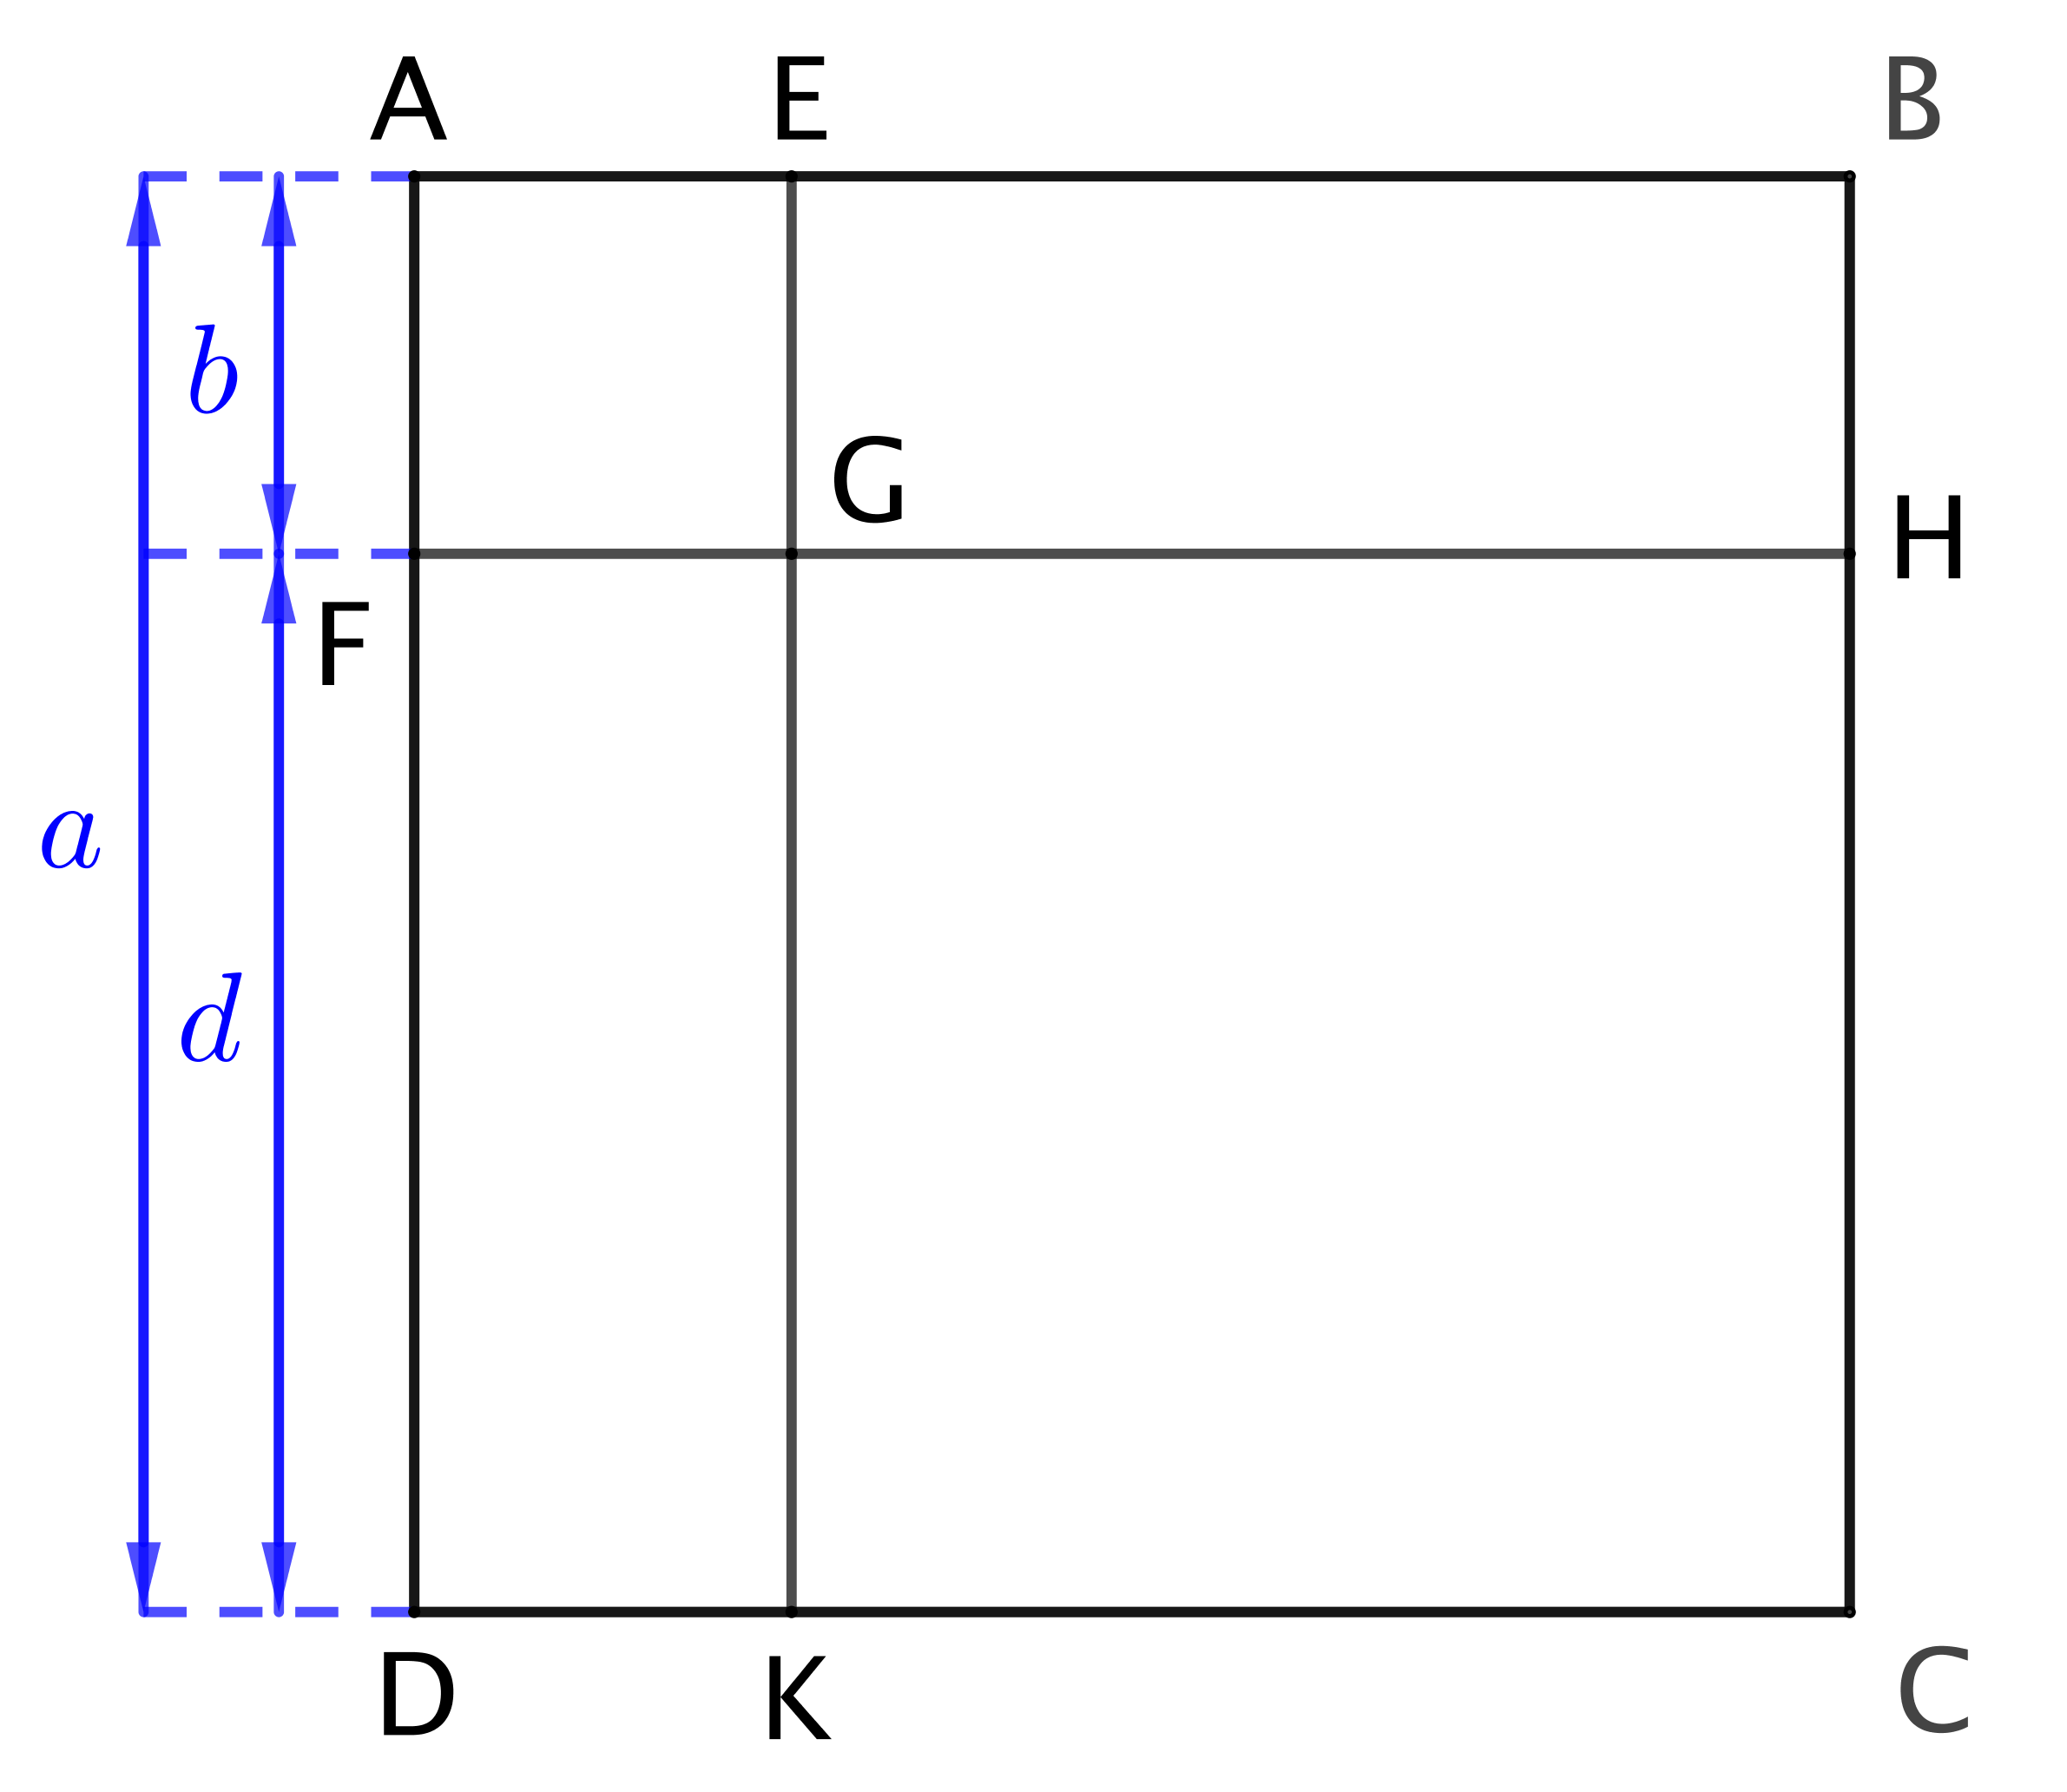
\includegraphics[scale = .7]{(a-b)^2.png}
\end{center}

Le fait \ref{poly-nullity-pos}, bien que très utile, ne peut plus s'appliquer ici au calcul géométrique évident suivant.

\leavevmode\kern-1em%
\begin{stepcalc}[style=ar*, ope={\iff}]
    \setgeo*{A}{GHCK} = \setgeo*{A}{ABCD} - \setgeo*{A}{ABHF} - \setgeo*{A}{AEKD} + \setgeo*{A}{AEGF}
\explnext{}
    (a-b)^2 = a^2 - 2ab + b^2
\end{stepcalc}

Peut-on tout de même déduire du calcul géométrique précédent la validité, pour tous les réels $a$ et $b$, de l'identité $(a - b)^2 = a^2 + b^2 - 2ab$?
Le fait \ref{poly-nullity-interval} suivant montre que cela est possible. 


\medskip

\begin{fact} \label{poly-nullity-interval}
	Soit $p: \RR^n \rightarrow \RR$ une fonction polynomiale à $n$ variables, où $n \in \NNs$.
	Si $\setgeo{E} \subseteq \RR^n$ contient $\setgeo*{E}{1} \times \cdots \times \setgeo*{E}{n}$ où chaque $\setgeo*{E}{k} \subseteq \RR$ est infini,
	et si $p$ s'annule sur $\setgeo{E}$,
	alors $p$ s'annule sur $\RR^n$ tout entier. 
\end{fact}


\begin{proof}
	La preuve du fait \ref{poly-nullity-pos} s'adapte facilement au cadre proposé ici.
\end{proof}


% ----------- %


\medskip

\begin{example}
Considérons le dessin ci-dessous avec $d = a - b$, et la contrainte $a > b$.

\begin{center}
	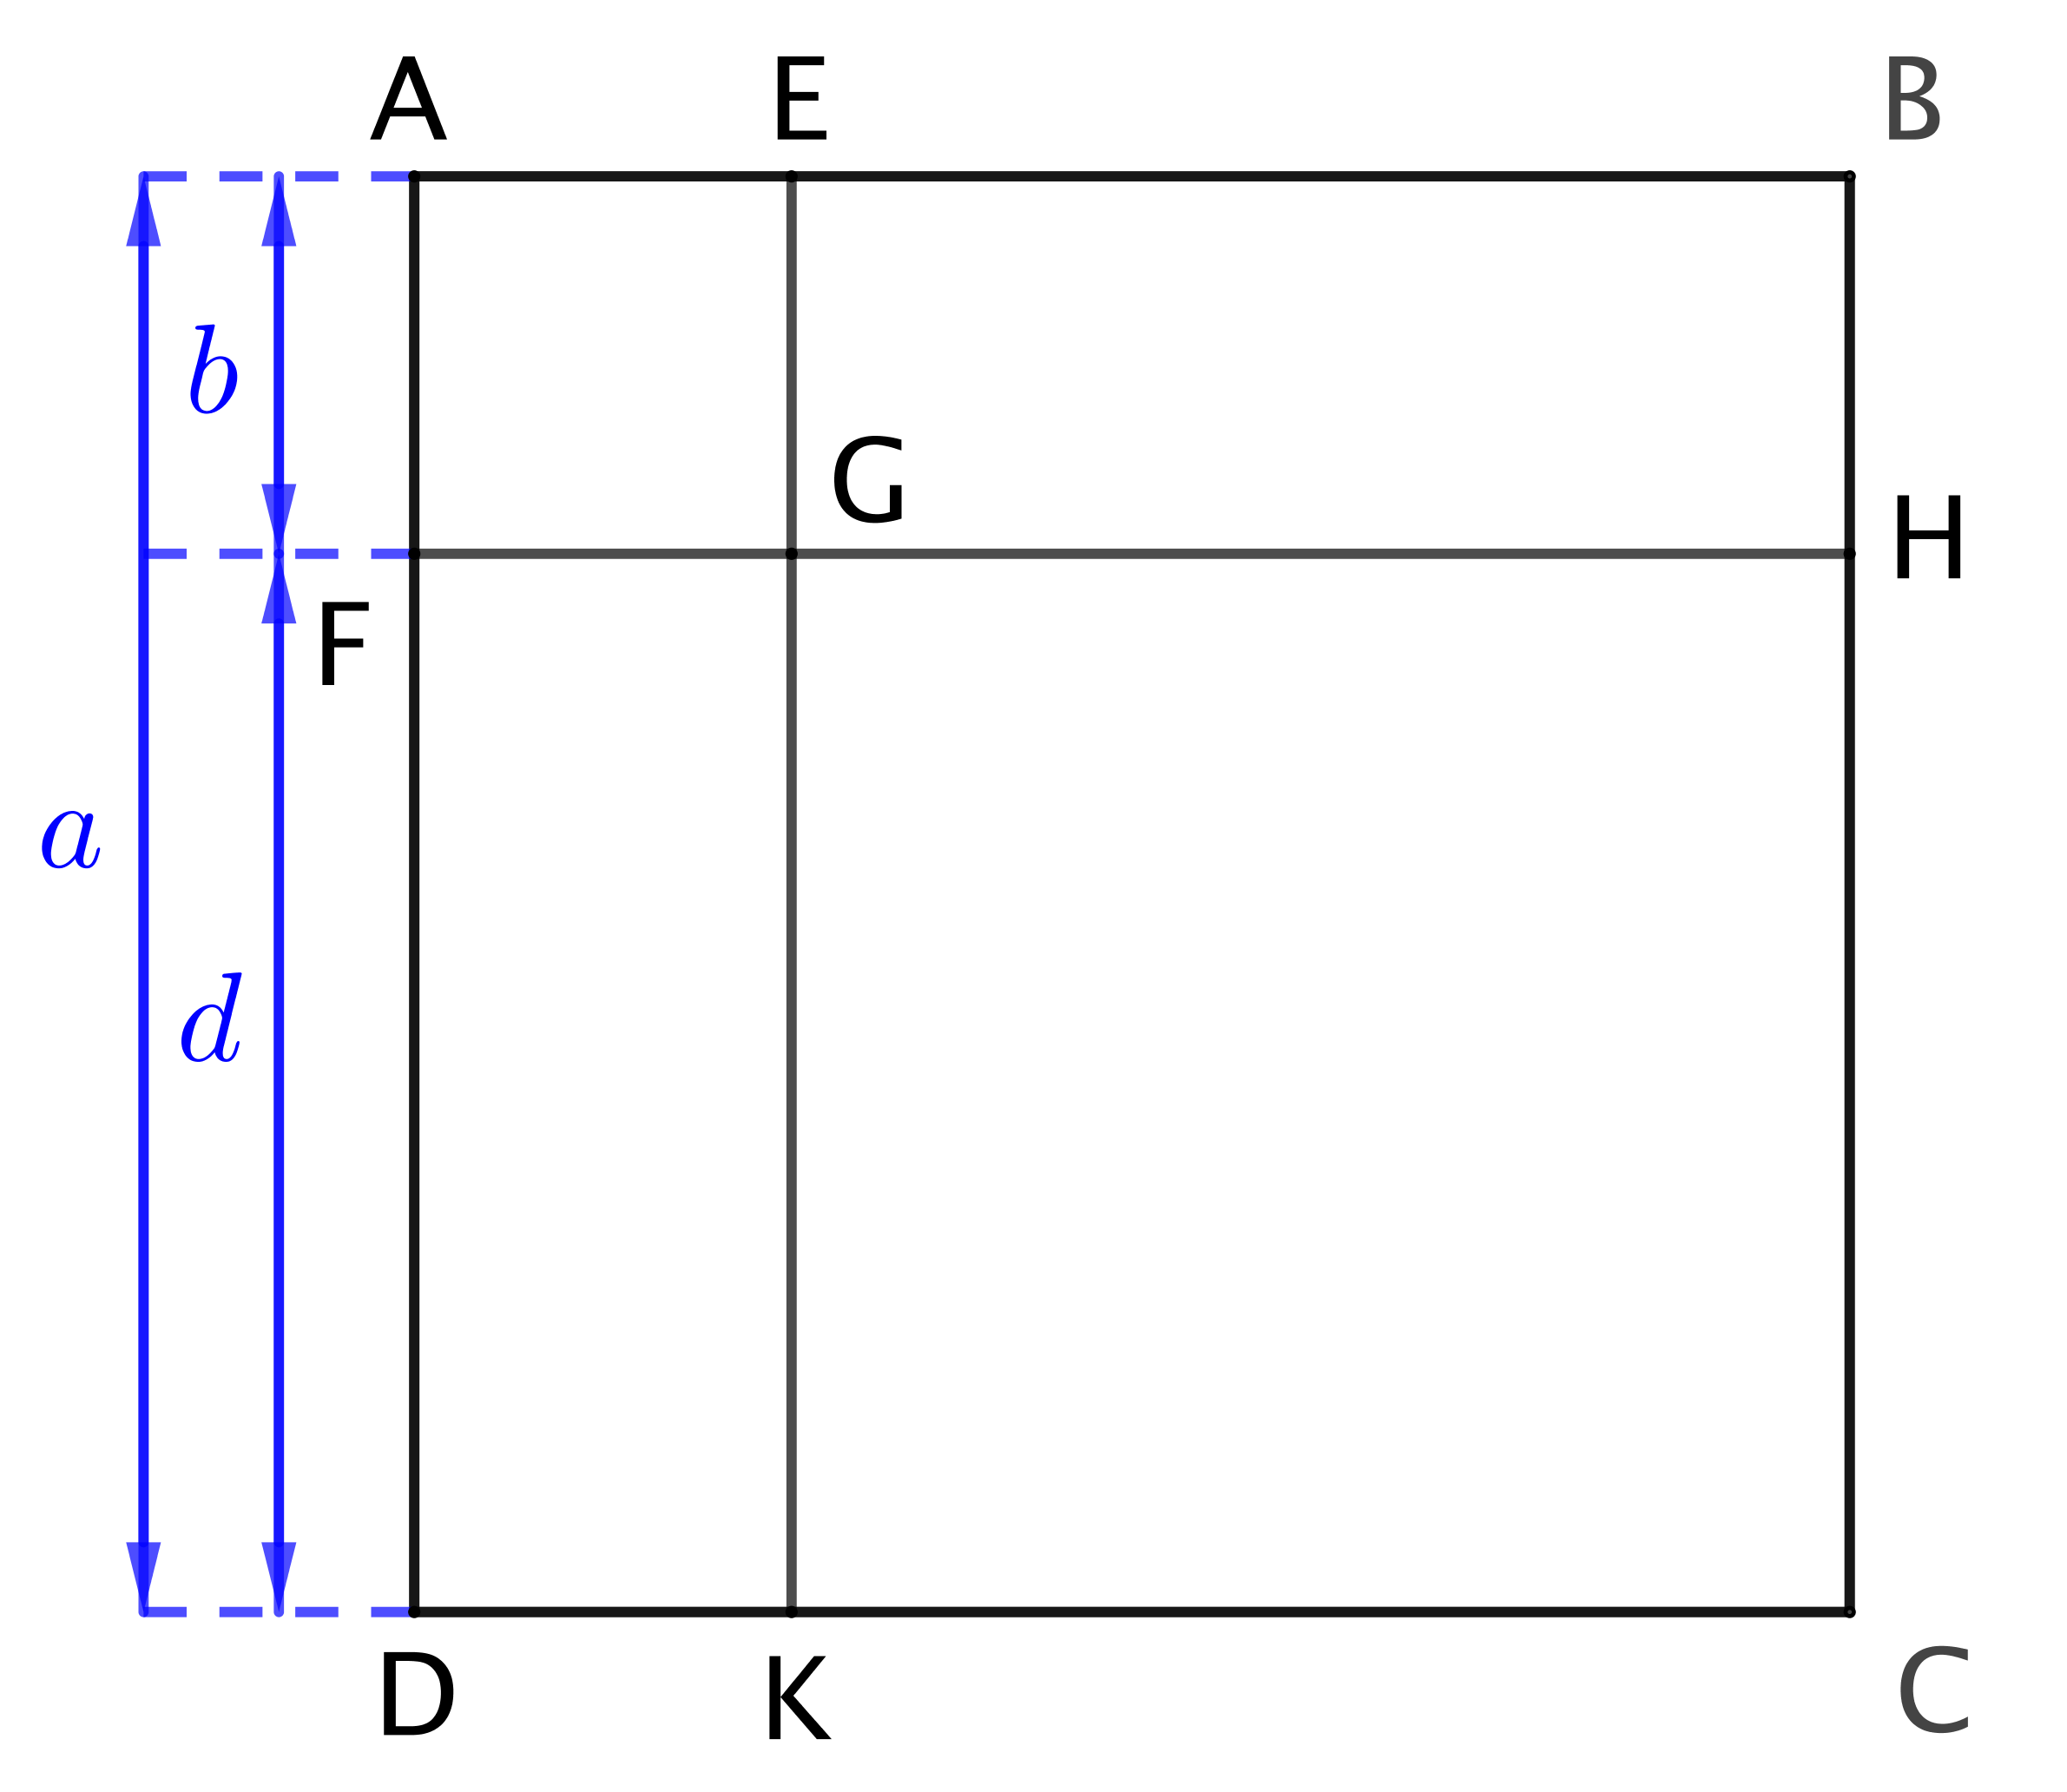
\includegraphics[scale = .7]{(a-b)^2.png}
\end{center}

Nous avons les calculs géométriques simples suivants.

\leavevmode\kern-1em%
\begin{stepcalc}[style=ar*, ope={\iff}]
    \setgeo*{A}{ABCD} - \setgeo*{A}{AEGF} = \setgeo*{A}{GHCK} + \setgeo*{A}{EBHG} + \setgeo*{A}{FGKD}
\explnext{}
    a^2 - b^2 = \setgeo*{A}{GHCK} + \setgeo*{A}{EBHG} + \setgeo*{A}{FGKD}
\end{stepcalc}

En déplaçant ensuite le rectangle $EBHG$ comme ci-dessous, nous obtenons alors un rectangle de dimension $(a+b) \times (a-b)$. 
	
\begin{center}
	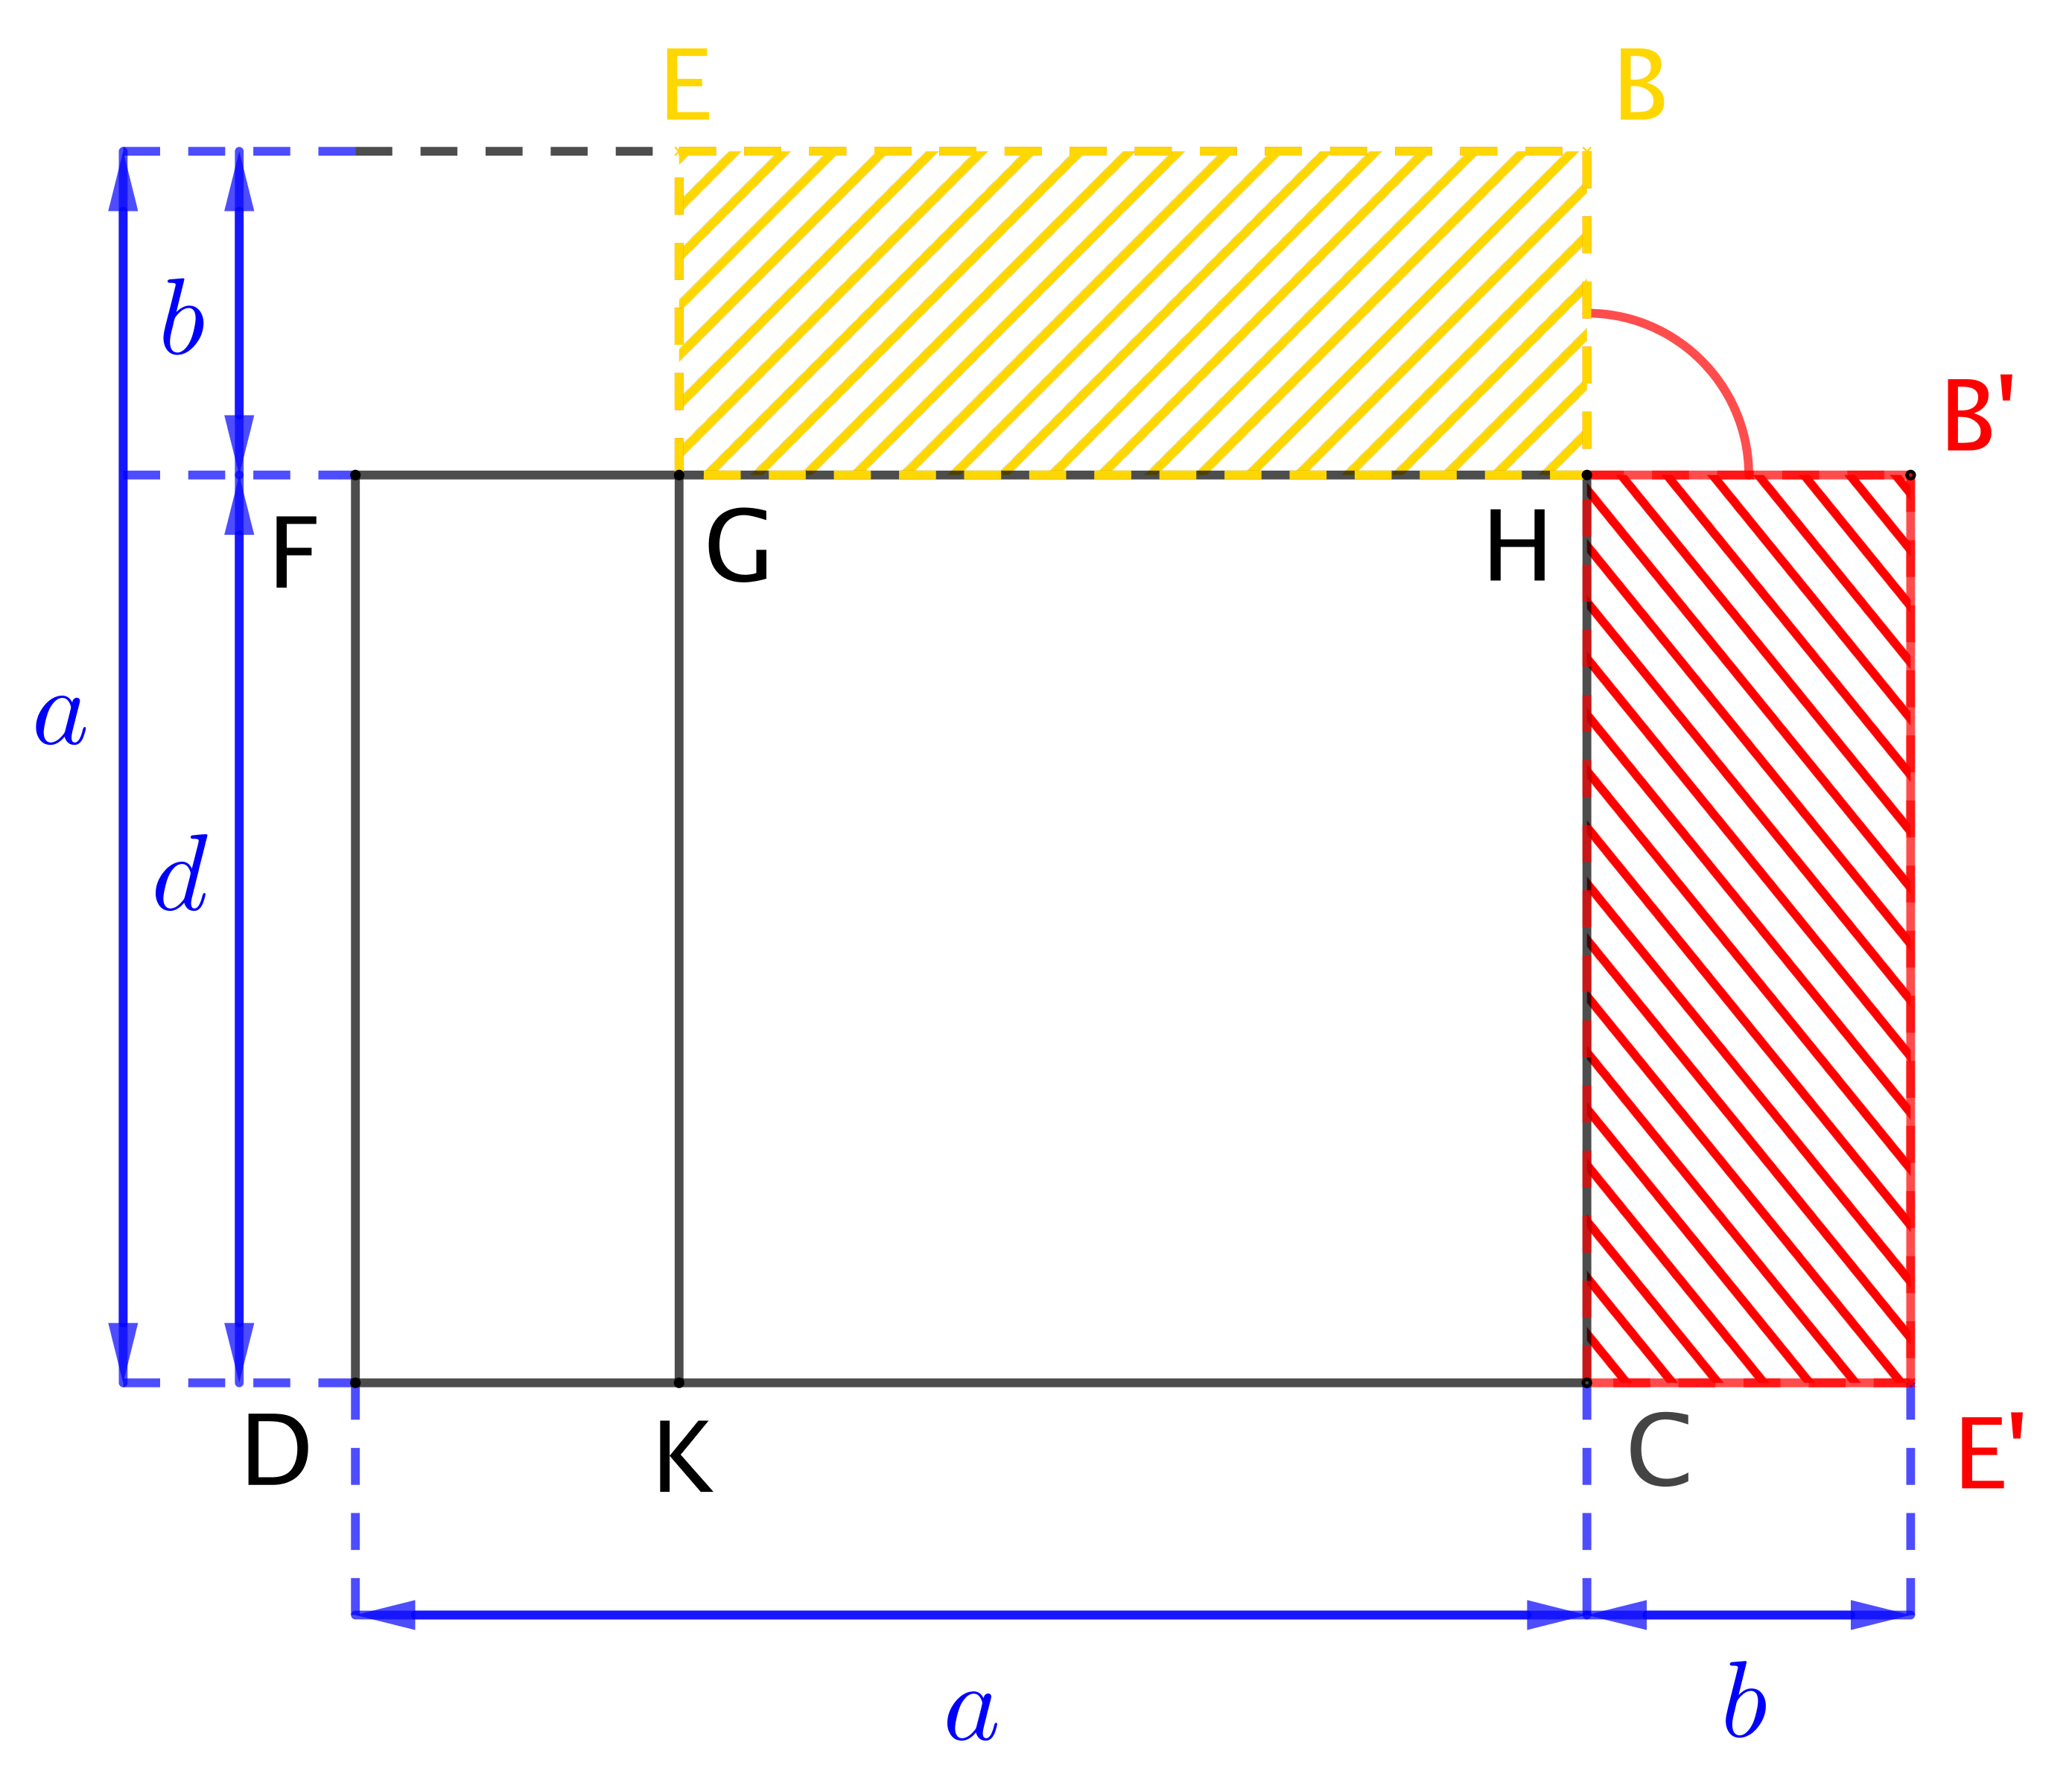
\includegraphics[scale = .7]{(a-b)(a-b)-spe.png}
\end{center}

Finalement, nous obtenons $a^2 - b^2 = (a+b)(a-b)$ si $a > b$,
puis, 
en appliquant le fait \ref{poly-nullity-interval} à $p(a ; b) = a^2 - b^2 - (a+b)(a-b)$, 
on obtient: $\forall (a ; b) \in \RR^2$, $a^2 - b^2 = (a+b)(a-b)$.
\end{example}
